\documentclass[11pt]{article}
%\usepackage[14pt]{extsizes} % для того чтобы задать нестандартный 14-ый размер шрифта
%\usepackage[utf8]{inputenc}
\usepackage{mathtext}
\usepackage[english, russian]{babel}
\usepackage{amsmath}
\usepackage{amsfonts}
\usepackage{float}
\usepackage[margin=0.8in]{geometry}
\usepackage{multirow}
\usepackage{graphicx}
\usepackage[utf8x]{inputenc} % указать кодировку русского текста
\usepackage{fancyhdr}
\usepackage{indentfirst} % отступ в первой строке абзаца
\usepackage{wrapfig}
\usepackage{placeins}
\usepackage{caption}
\usepackage{amssymb}
\usepackage{mathtools}
\usepackage[thinc]{esdiff}
\usepackage{cmap}
\usepackage[table,xcdraw]{xcolor}
\usepackage{amsmath,amsfonts,amssymb,amsthm,mathtools, mathrsfs}
\usepackage{breqn}
\usepackage{subcaption}

\pagestyle{fancy}
\begin{document}
\begin{titlepage}
\begin{center}
%\vspace*{1cm}
\large{\small ФЕДЕРАЛЬНОЕ ГОСУДАРСТВЕННОЕ АВТОНОМНОЕ ОБРАЗОВАТЕЛЬНОЕ\\ УЧРЕЖДЕНИЕ ВЫСШЕГО ОБРАЗОВАНИЯ\\ МОСКОВСКИЙ ФИЗИКО-ТЕХНИЧЕСКИЙ ИНСТИТУТ\\ (НАЦИОНАЛЬНЫЙ ИССЛЕДОВАТЕЛЬСКИЙ УНИВЕРСИТЕТ)\\ ФИЗТЕХ-ШКОЛА РАДИОТЕХНИКИ И КОМПЬЮТЕРНЫХ ТЕХНОЛОГИЙ}
\vfill
\line(1,0){430}\\[1mm]
\huge{Лабораторная работа 3.3.4}\\
\huge\textbf{Эффект Холла в полупроводниках.}\\
\line(1,0){430}\\[1mm]
\vfill
\begin{flushright}
\normalsize{Устюжанина Мария}\\
\normalsize{\textbf{Группа Б01-107}}\\
\end{flushright}
\end{center}
\end{titlepage}
\fancyhead[L] {Работа 3.3.4}

\par \textbf{Цель работы:} измерение подвижности и конуентрации носителей заряда в проводниках.

\par \textbf{В работе используются:} электромагнит с регулируемым источником питания; вольтетр; амперметр; миллиамперметр; милливебберметр; источник питания (1.5 В); Образец легированного германия.



\section{Теоретическая справка}
    Суть эффекта Холла состоит в следующем. Пусть через однородную пластину металла вдоль оси $x$ течет ток $I$ (рис. 1).
    
    \begin{wrapfigure}{l}{0.6\textwidth}
        \vspace{-20pt}
        \begin{center}
            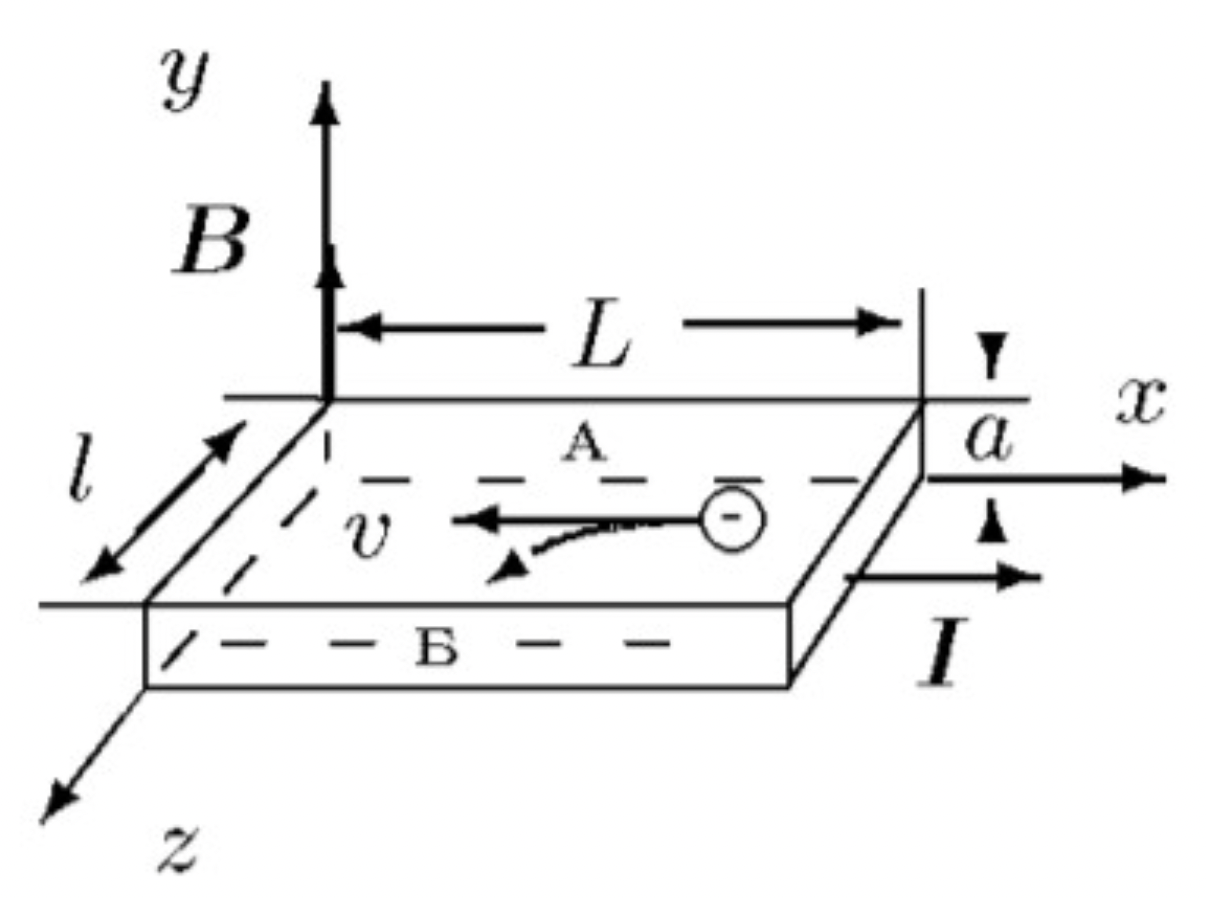
\includegraphics[width=0.7\linewidth]{holl.jpg}
            \label{fig:sdfsafd}
        \end{center}
        \vspace{-20pt}
        \caption{Образец с током в магнитном поле}
    \end{wrapfigure}

    Если эту пластину поместить в магнитное поле, направленное по оси y, то между гранями А и Б появляется разность потенциалов. 
    
    В самом деле, на электрон (для простоты рассматриваем один тип носителей), движущийся со средней скоростью $\langle \vec{v} \rangle$ в электромагнитном поле, действует сила Лоренца:
    
    $$\vec{F}_{л} = -e\vec{E}-e \langle \vec{v} \rangle \times \vec{B},$$
    
    где $e$- абсолютный заряд электрона, $\vec{E}$ - напряженность электрического поля, $\vec{B}$ - индукция магнитного поля.
    
    В проекции на ось $z$ получаем
    
    $$ F_{B}=e | \langle {v_{x}} \rangle | B.$$
    
    Под действием этой силы электроны отклоняются к грани Б, заряжая ее отрицательно. На грани А накапливаются нескомпенсированные положительные заряды. Это приводит к возникновению электрического поля $E_{z}$, направленного от А к Б, которое действует на электроны с силой $F_{E}=eE_{z}$. В установившемся режиме $F_{E}=F_{B}$, поэтому накопление электрических зарядов на боковых гранях пластины прекращается. Отсюда
    
    $$ E_{z}=| \langle {v_{x}} \rangle | B.$$
    
    С этим полем связана разность потенциалов $$U_{AБ}=E_{z}l=| \langle {v_{x}} \rangle | Bl.$$
    
    В этом и состоит эффект Холла.
    
    \
    
    Замечая, что сила тока
    
    $$ I=ne| \langle {v_{x}} \rangle |la,$$
    
    найдем ЭДС Холла:
    
\begin{equation}\label{Rx}
    \mathscr{E}_{X}=U_{AБ}=\dfrac{IB}{nea}=R_{X}\dfrac{IB}{a}
\end{equation}
    
    Константа $R_{X}=\dfrac{1}{ne}$ называется постоянной Холла.
    
    В полупроводниках, когда вклад в проводимость обусловлен и электронами и дырками, выражение для постоянной Холла имеет более сложный вид:
    
    $$R_{X}=\dfrac{nb^{2}_{e}-pb^{2}_{p}}{e(nb_{e}+pb_{p})^{2}},$$
    
    где $n$ и $p$ - концентрации электронов и дырок, $b_{e}$ $b_{p}$ - их подвижности.
    




\section{Экспериментальная установка}
    \begin{figure}[H]
    \center{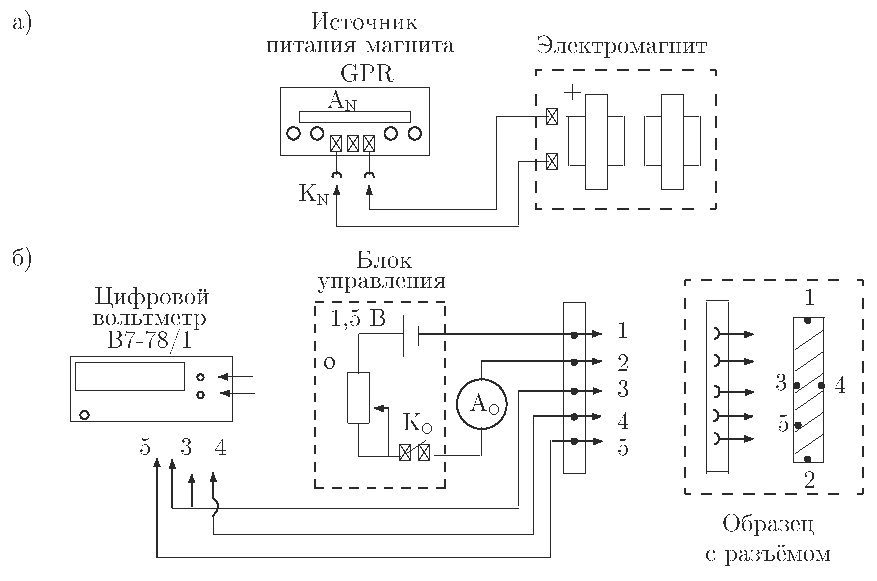
\includegraphics[scale=0.7]{ustanovka.pdf}}
    \caption{Электрическая установка для измерения ЭДС Холла.}
    \label{pic:3}
    \end{figure}
\newpage




\section{Ход работы:}

\textbf{Нacтроим приборы}

1) Построим калибровочную кривую электромагнита (параметр милливебберметра \( S\cdot N = 72 см^2 \)): 

\begin{table}[H]
    \centering
    \begin{tabular}{|c|c|}
        \hline
        I, A  & B, Тл  \\\hline
        0.27  & 0.21  \\\hline
        0.54  & 0.42  \\\hline
        0.81  & 0.625 \\\hline
        1.08  & 0.79  \\\hline
        1.35  & 0.94  \\\hline
        1.62  & 1.04  \\\hline
        1.89  & 1.125 \\\hline
        2.13  & 1.16  \\\hline  
    \end{tabular}
\end{table}

\begin{figure} [H]
    \centering
    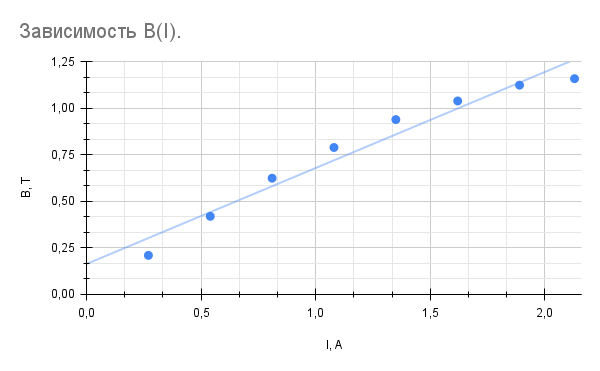
\includegraphics[width=\textwidth]{graf1.png}
\end{figure}

2) Вычислим зависимость:

\[ B = ((0.52 \pm 0.04) Тл/A) \cdot I + (0.16 \pm 0.02) Тл  \]

Вставим образец в зазор выключенного электромагнита и определим начато отсчета напряжения  (\( U_0 = -0.017 \) В) между Холловскими кантактами при минимальном точке через образец (\( I = 0.3 \) мА).

\textbf{Измереним ЭДС Холла}

Получим зависимость холловского напряжения \(U_{34}\) от тока через электромагнит \(I_{M}\) для разных токов \(I\) через образец:

\begin{figure}[H]
    \centering
    \begin{subfigure}{.5\textwidth}
    \centering
    \begin{tabular}{|c|c|c|c|}
        \hline
        I, мА & U0, мВ & Iм, A & U34, мВ \\\hline
        & & 0.27 & -0.04  \\
        & & 0.54 & -0.065 \\
        & & 0.81 & -0.089 \\
        & & 1.08 & -0.111 \\
        & & 1.35 & -0.130 \\
        & & 1.62 & -0.140 \\
        & & 1.89 & -0.150 \\
        \multirow{-8}{*}{0.3}         & \multirow{-8}{*}{-0.017}       & 2.11 & -0.155 \\\hline
        & & 0.27 & 0.013  \\
        & & 0.54 & 0.044  \\
        & & 0.81 & 0.074  \\
        & & 1.08 & 0.102  \\
        & & 1.35 & 0.123  \\
        & & 1.62 & 0.138  \\
        & & 1.89 & 0.148  \\
        \multirow{-8}{*}{0.4}         & \multirow{-8}{*}{-0.017}       & 2.08 & 0.153  \\\hline
        & & 0.27 & 0.013  \\
        & & 0.54 & 0.052  \\
        & & 0.81 & 0.094  \\
        & & 1.08 & 0.127  \\
        & & 1.35 & 0.152  \\
        & & 1.62 & 0.170  \\
        & & 1.89 & 0.183  \\
        \multirow{-8}{*}{0.5} & \multirow{-8}{*}{-0.025}       & 2.07 & 0.190  \\\hline
        & & 0.27 & 0.016  \\
        & & 0.54 & 0.064  \\
        & & 0.81 & 0.110  \\
        & & 1.08 & 0.151  \\
        & & 1.35 & 0.184  \\
        & & 1.62 & 0.205  \\
        & & 1.89 & 0.220  \\
        \multirow{-8}{*}{0.6}         & \multirow{-8}{*}{-0.03}        & 2.06 & 0.228  \\\hline
    \end {tabular}
    \end{subfigure}%
    \begin{subfigure}{.5\textwidth}
        \centering
    \begin{tabular}{|c|c|c|c|}
        \hline
        I, мА & U0, мВ & Iм, A & U34, мВ \\\hline
        & & 0.27 & 0.017  \\
        & & 0.54 & 0.074  \\
        & & 0.81 & 0.128  \\
        & & 1.08 & 0.175  \\
        & & 1.35 & 0.214  \\
        & & 1.62 & 0.240  \\
        & & 1.89 & 0.257  \\
        \multirow{-8}{*}{0.7}         & \multirow{-8}{*}{-0.037}       & 2.04 & 0.265  \\\hline
        & & 0.27 & 0.019  \\ 
        & & 0.54 & 0.086  \\ 
        & & 0.81 & 0.145  \\ 
        & & 1.08 & 0.203  \\ 
        & & 1.35 & 0.240  \\ 
        & & 1.62 & 0.270  \\ 
        & & 1.89 & 0.292  \\ 
        \multirow{-8}{*}{0.8}         & \multirow{-8}{*}{-0.042}       & 2.04 & 0.3    \\\hline
        & & 0.27 & 0.022  \\ 
        & & 0.54 & 0.096  \\ 
        & & 0.81 & 0.165  \\ 
        & & 1.08 & 0.222  \\ 
        & & 1.35 & 0.275  \\ 
        & & 1.62 & 0.306  \\ 
        & & 1.89 & 0.328  \\ 
        \multirow{-8}{*}{0.9}         & \multirow{-8}{*}{-0.05}        & 2.03 & 0.339  \\\hline
        & & 0.27 & 0.027  \\ 
        & & 0.54 & 0.103  \\ 
        & & 0.81 & 0.180  \\ 
        & & 1.08 & 0.250  \\ 
        & & 1.35 & 0.302  \\ 
        & & 1.62 & 0.340  \\ 
        & & 1.89 & 0.365  \\ 
        \multirow{-8}{*}{1}           & \multirow{-8}{*}{-0.055}       & 2.03 & 0.375 \\\hline
        \end{tabular}
    \end{subfigure}%
\end{figure}

Построим графики \(U(B)\) на одном чертеже:

\begin{figure}[H]
    \centering
    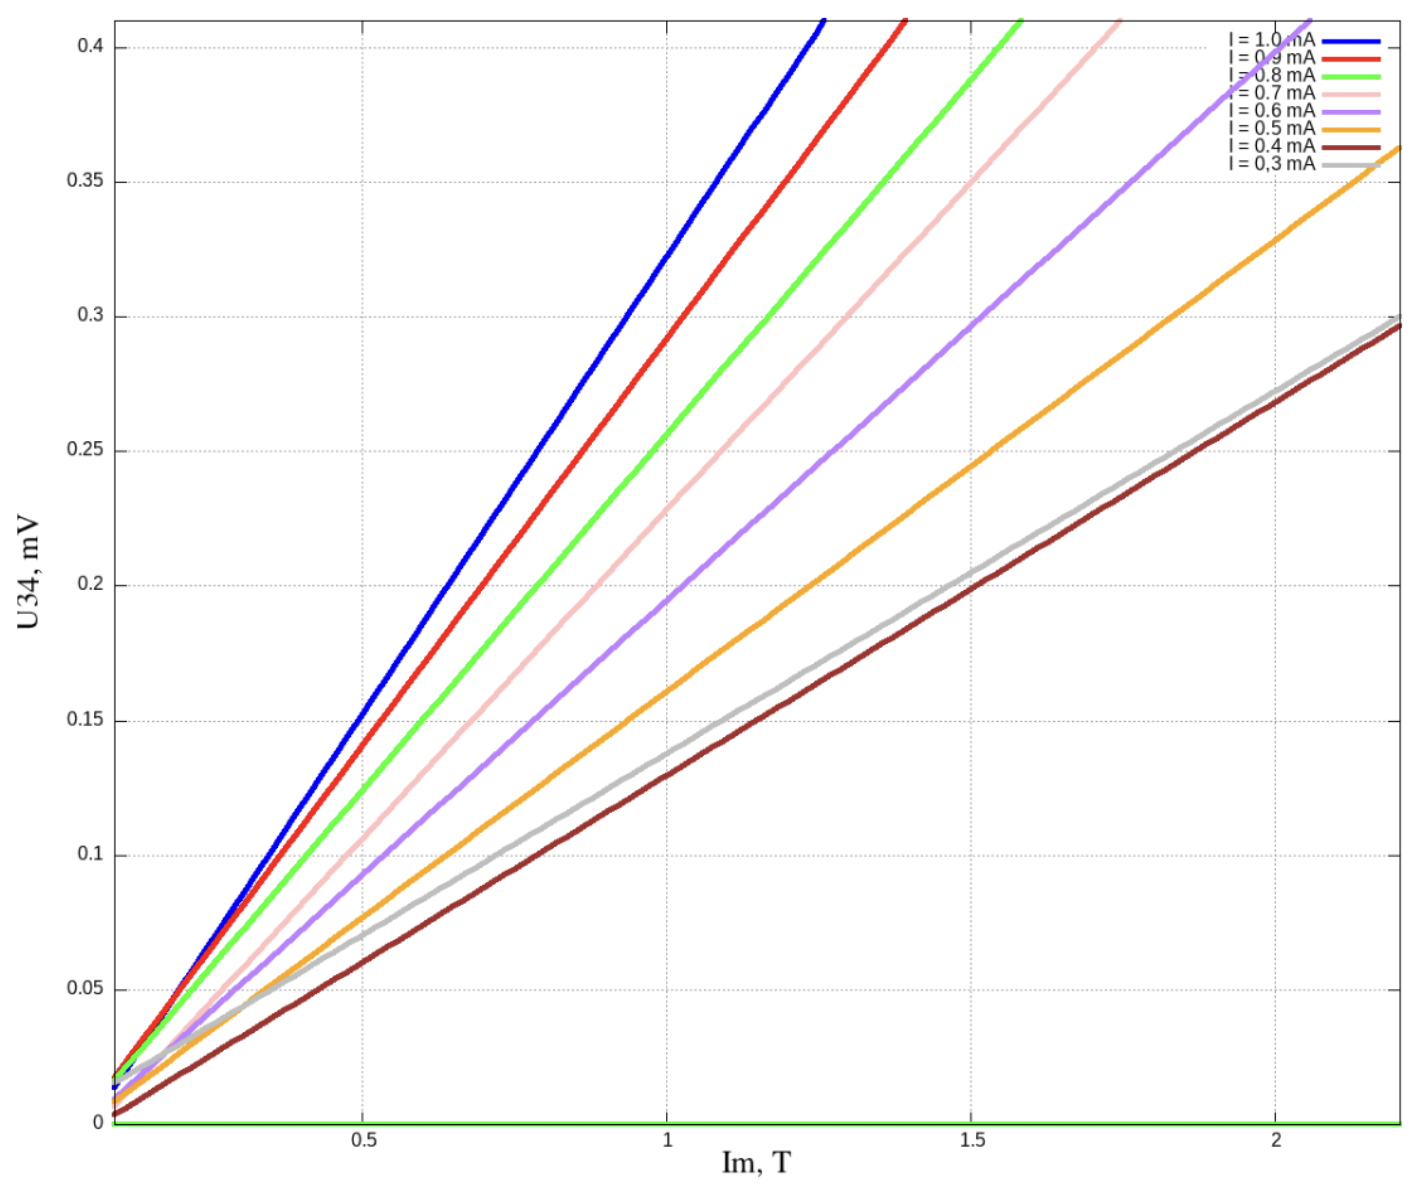
\includegraphics[width=\textwidth]{graf2.png}
\end{figure}
    

По МНК получим линейную зависимость \( U = k \cdot B + b \). Полученные коэффициенты:

\begin{table}[H]
    \centering
    \begin{tabular}{|c|c|}
        \hline
        \( I, мА \) & \( k, мВ/Тл \)\\\hline
        0.3 & \( 0.135 \pm 0.006 \) \\\hline
        0.4 & \( 0.139 \pm 0.007 \) \\\hline
        0.5 & \( 0.168 \pm 0.008 \) \\\hline
        0.6 & \( 0.204 \pm 0.01  \) \\\hline
        0.7 & \( 0.244 \pm 0.01  \) \\\hline
        0.8 & \( 0.264 \pm 0.007 \) \\\hline
        0.9 & \( 0.302 \pm 0.011 \) \\\hline
        1.0 & \( 0.340 \pm 0.015 \) \\\hline
    \end{tabular}
\end{table}

Получим заыисимость \( k(B) \):

\begin{figure}[H]
    \centering
    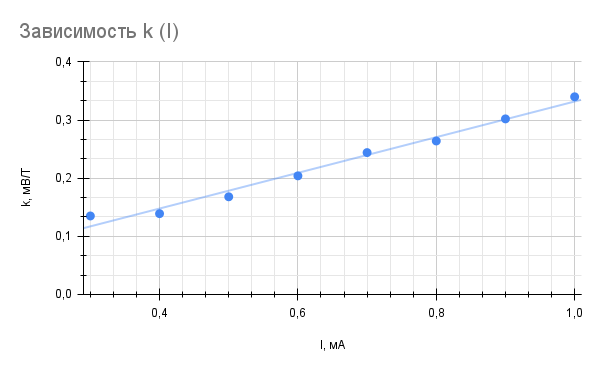
\includegraphics[width=\textwidth]{graf3.png}
\end{figure}

Аппроксимируем: \( k = (0.31 \pm 0.014) \frac{В}{Тл\cdot A}  \cdot I + (0.025 \pm 0.003) мВ/Тл \), где

По формуле:
\[ a = \frac{U34}{B\cdot I} = \frac{R_H}{h} \]

Вычислим постоянную Холла (Учитывая \(h = 1.5 mm\)):
\[ R_H = a\cdot h = (0.47 \pm 0.02) \; 10^{-3}\frac{В\cdot m}{Тл\cdot A} \]

А по формуле:
\[ R_H = \frac{1}{n\cdot e} \]

Получим значение концентрации \(n\) свободных носителей заряда в образце:
\[ n = (1.33 \pm 0.31)\; 10^{-22}m^{-3} \]

Найдем удельную проводимость образца. По формуле:
\[ \sigma = \frac{I\cdot L_{35}}{U_{35}al} \]
Взяв изначения (\( I = 1.0\; мА, U_{35} = 1.681\; мВ \)), учтем параметры образца (\(L_{35} = 3.0\; mm, h = 1.5\; mm, l = 1.7\; mm\)), получим:

\[ \sigma = (699.8 \pm 81)\; (\Omega\cdot m)^{-1} \]

Найдем подвижность носителей заряда по формуле:
\[ b = \frac{\sigma}{en} = \sigma\cdot R_H = (3285 \pm 395)\; \frac{см^2}{В\cdot s} \]

\section{Выводы}

В работы мы исследовали эффект Холла в легированном германии (полупроводник). Были экспериментально получены постоянная Холла для исследуемого образца
\( R_H = (0.47 \pm 0.02)\; 10^{-3} \frac{В\cdot m}{Тл\cdot A} \) и концентрация свободных носителей заряда
\( n = n = (1.33 \pm 0.31)\; 10^{-22}m^{-3} \). Мы измерели удельная проводимость образца: \\
\( \sigma = (699.8 \pm 81)\; (\Omega\cdot m)^{-1} \).
    
По направлению тока в образце и направлению силовых линий электромагнита можно заключить, что
образец обладает электронной проводимостью. В работе рассчитали подвижность носителей заряда в образце:
\( b = (3285 \pm 395)\; \frac{см^2}{В\cdot s} \). Полученный результат отличается от табличного значения
\( b_0 = 3900 \frac{см^2}{В\cdot s} \), но не очень сильно. Возможно, это из-за неточности измерения приборов из-за нагревы и наличия примесей в образце.


\end{document}